\documentclass[10pt]{article}
\usepackage[margin=1in]{geometry} 
\usepackage{enumerate, xfrac, color, graphicx}
\usepackage{amsmath,amsthm,amssymb,amsfonts,mathabx}
\usepackage{booktabs}
\usepackage{caption}
\usepackage{algorithm}
\usepackage{algpseudocode}
\usepackage{pifont}
\usepackage{listings, courier}
\graphicspath{{/Users/mfzhao/Dropbox/}}
\newcommand{\N}{\mathbb{N}}
\newcommand{\Z}{\mathbb{Z}}
\lstset{breaklines=true, basicstyle=\small\ttfamily, language=R, backgroundcolor=\color{highlight}, stepnumber=5}

\definecolor{highlight}{RGB}{248,248,248}

\begin{document}
	\title{6.867 Problem Set 2}
	\maketitle


\subsubsection*{Logistic Regression}
Here we want to predict the class of a discrete (or categorical) variable $Y$ given some some features $X$. While we can formulate this classification problem in the context of the linear regression framework we're already familiar with (these are known as linear probability models), these classical linear models are generally unbounded which may not be the best choice for modeling probabilities. Rather, we consider a slightly modified version of linear regression where we take the standard linear prediction $w_o + \sum_i w_i x_i$ and transform it such that it is bounded on $[0,1]$. In our case, our choice of a transformation function is the sigmoid function:
\begin{equation*}
	\sigma(z) = \frac{1}{1+e^{z}}
\end{equation*}

This transformed model is known as logistic or logit regression. Using this formulation, our the negative log-likelihood becomes:
\begin{equation*}
	\textnormal{NLL}=\sum_i \log \left(1+e^{-y^{(i)}(w_0 + x^{(i)}\cdot w)} \right)
\end{equation*}
We think that overfitting might be problem in logistic regression especially in the case of linearly separable data which will drive our weights $w$ to very large values to minimize the the logistic loss. Hence, we add a ridge penalty to the weights on the features to shrink them:
\begin{equation*}
	\min_w \sum_i \log \left(1+e^{-y^{(i)}(w_0 + x^{(i)}\cdot w)} \right) + \lambda w^T w
\end{equation*}
Using this, we trained Logistic Regressions for each of our 4 datasets using gradient descent. The optimal weights are reported below:

\begin{table}[ht]
\centering
\captionof{table}{Optimal Weights Trained on Various Datasets}
\begin{tabular}{lrrrr}
\toprule
{}    &      stdev1 &    stdev2 &    stdev4 & nonsep\\
\midrule
$w_0$ &  -63.930971 & -0.009267 & -0.046649 & 0.000597\\
$w_1$ &  266.198033 &  0.236279 &  0.763589 & -0.024737\\
$w_2$ &  160.999118 &  0.203428 &  1.114811 & -0.023726\\
\bottomrule
\end{tabular}
\end{table}

Logistic regression produces a predicted probability of a class rather than an actual classification. This means that we need to decide a decision boundary to minimizes our classifcation error. Considering we have symmetric loss, we intuitively might want our decision boundary to be 0.5 which produces the following error rates:

\begin{table}[ht]
\centering
\captionof{table}{Performance of Logistic Regression with Decision boundary of 0.5}
\begin{tabular}{lrrrr}
\toprule
{} & stdev1 & stdev2 & stdev4 & nonsep\\
\midrule
  Training Error   & 0.00\%  & 9.25\% &  26.00\% & 48.50\% \\
  Validation Error & 0.00\%  & 8.00\% &  24.75\% & 50.75\% \\
\bottomrule
\end{tabular}
\end{table}


These results make a lot of sense as we should expect the classification error to be 0 for the perfectly linearly separable case and get progressively worse as as the two classes overlap. In fact, in the nonseparable case, our classifier is no better (or even slightly worse) than random guessing! We can see this as we plot our decision boundary in X-space below:

\begin{figure}[ht]
	\centering
	\begin{minipage}[b]{.24\linewidth}
		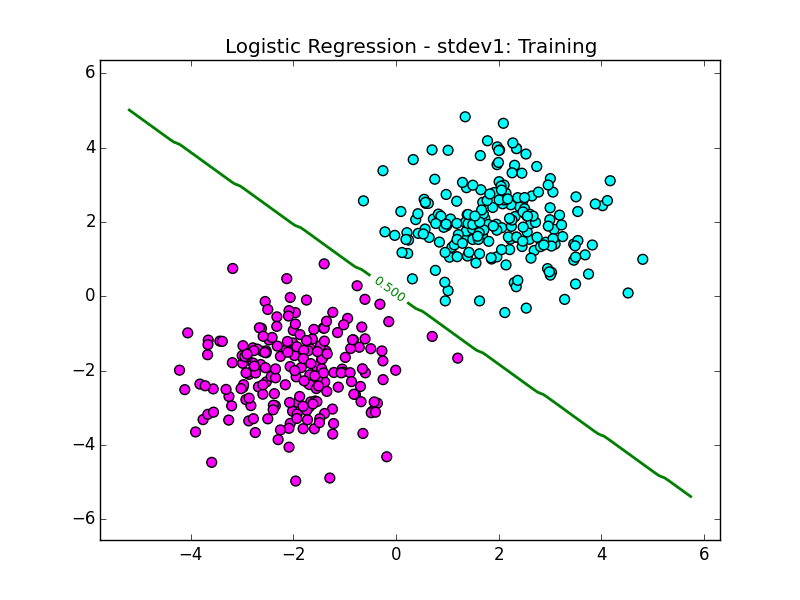
\includegraphics[width=1\linewidth, height=1in]{LR_stdev1_train.png}
		\caption*{stdev1 (Training)}
	\end{minipage}
	\begin{minipage}[b]{.24\linewidth}
		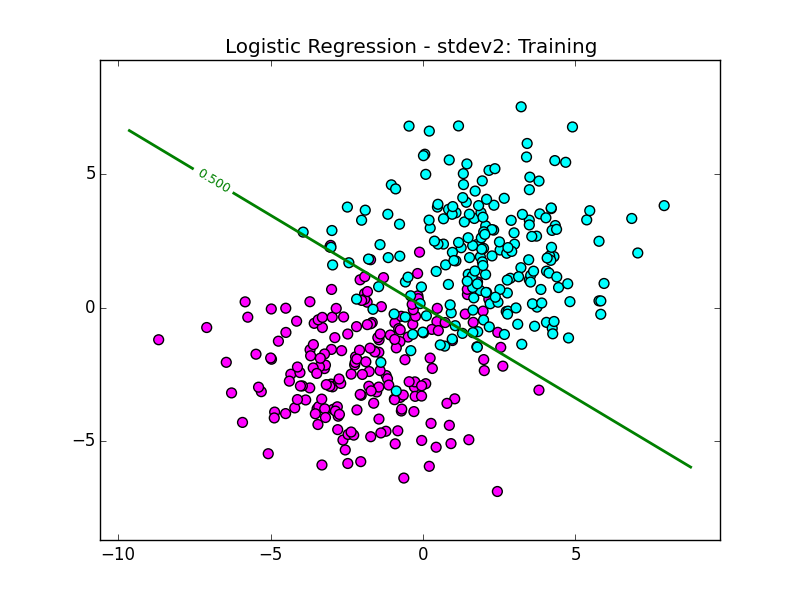
\includegraphics[width=1\linewidth, height=1in]{LR_stdev2_train.png}
		\caption*{stdev2 (Training)}
	\end{minipage}
	\begin{minipage}[b]{.24\linewidth}
		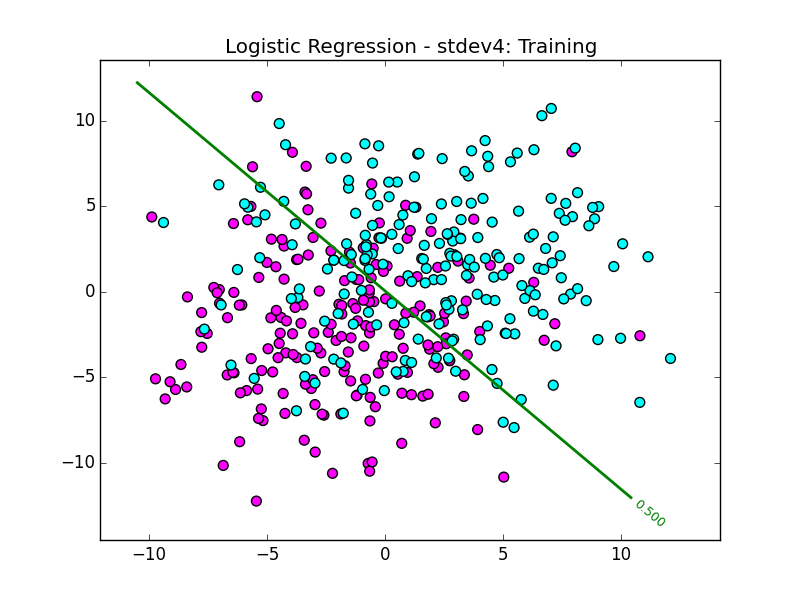
\includegraphics[width=1\linewidth, height=1in]{LR_stdev4_train.png}
		\caption*{stdev4 (Training)}
	\end{minipage}
	\begin{minipage}[b]{.24\linewidth}
		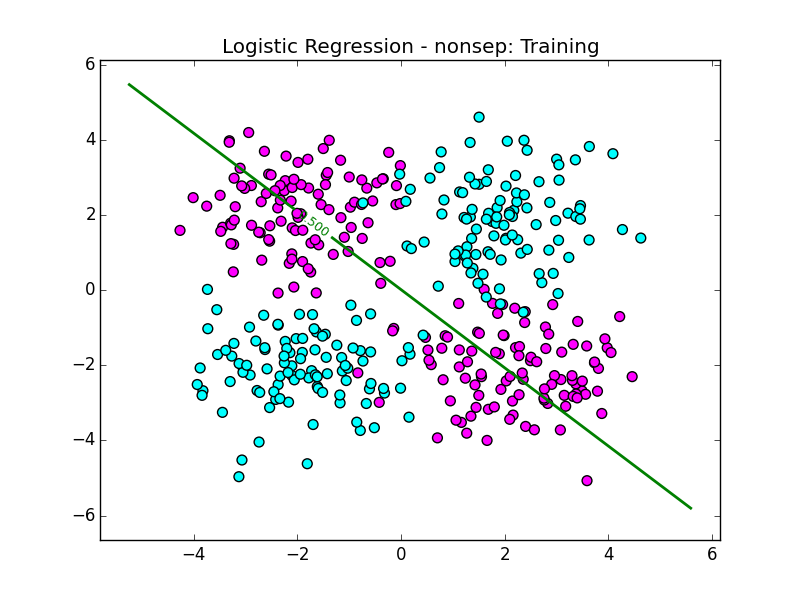
\includegraphics[width=1\linewidth, height=1in]{LR_nonsep_train.png}
		\caption*{nonsep (Training)}
	\end{minipage}
		\begin{minipage}[b]{.24\linewidth}
		\includegraphics[width=1\linewidth, height=1in]{LR_stdev1_validation.png}
		\caption*{stdev1 (Validation)}
	\end{minipage}
	\begin{minipage}[b]{.24\linewidth}
		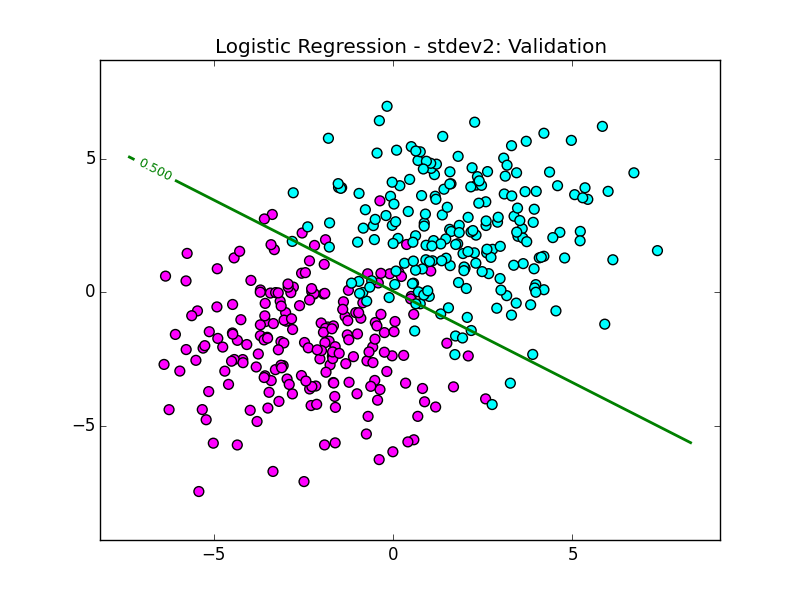
\includegraphics[width=1\linewidth, height=1in]{LR_stdev2_validation.png}
		\caption*{stdev2 (Validation)}
	\end{minipage}
	\begin{minipage}[b]{.24\linewidth}
		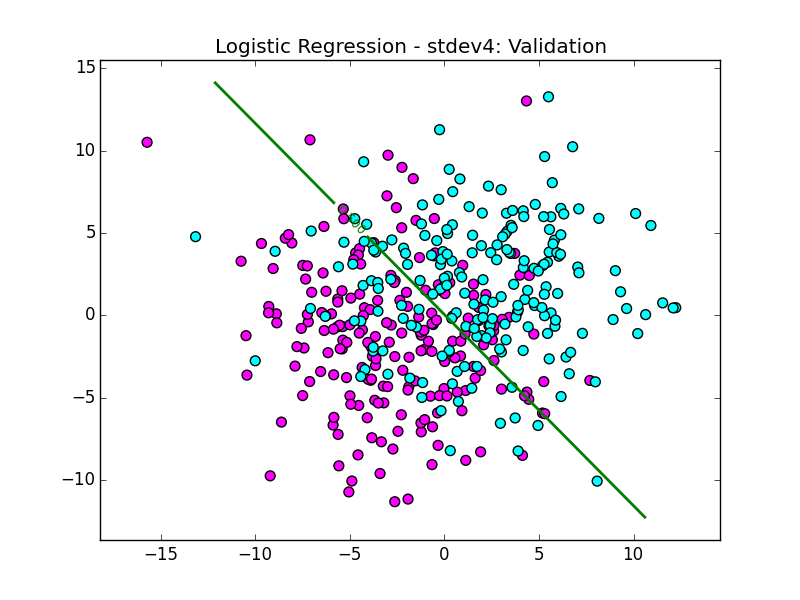
\includegraphics[width=1\linewidth, height=1in]{LR_stdev4_validation.png}
		\caption*{stdev4 (Validation)}
	\end{minipage}
	\begin{minipage}[b]{.24\linewidth}
		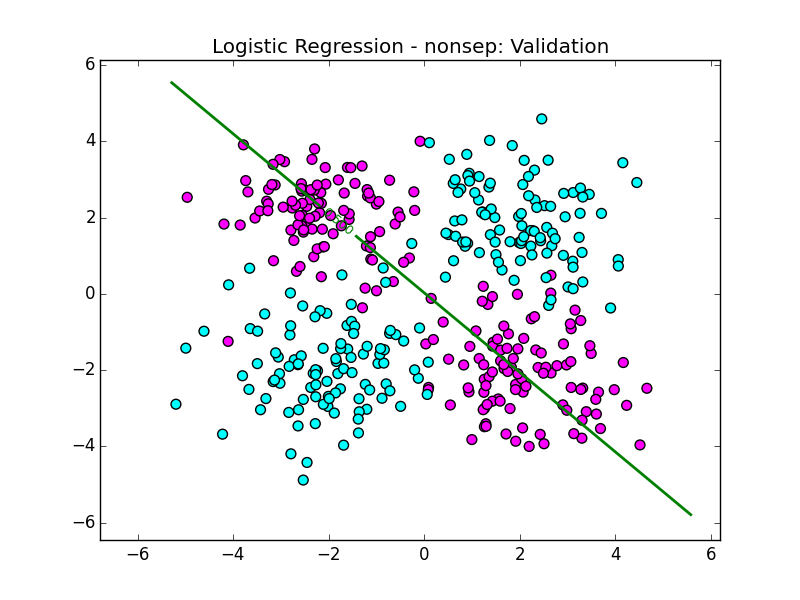
\includegraphics[width=1\linewidth, height=1in]{LR_nonsep_validation.png}
		\caption*{nonsep (Validation)}
	\end{minipage}
	\caption{The decision boundaries generated by Logistic Regression plotted against the stdev1, stdev2, stdev4, and nonsep (training and validation) datasets}
\end{figure}

We are also interested in examining classification error as we vary our choice of the decision boundary. This is depicted in in figure 2 below:

\begin{figure}[ht]
	\centering
	\begin{minipage}[b]{.24\linewidth}
		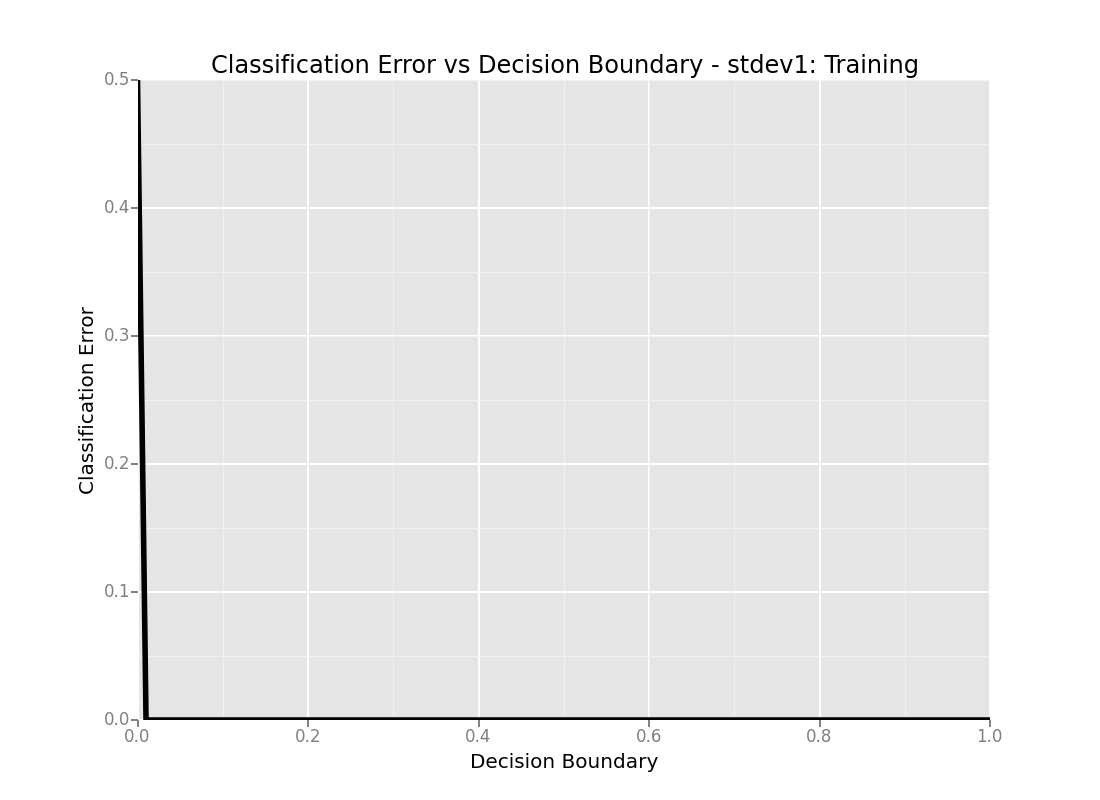
\includegraphics[width=1\linewidth, height=1in]{CEDB_stdev1_train.png}
		\caption*{stdev1 (Training)}
	\end{minipage}
	\begin{minipage}[b]{.24\linewidth}
		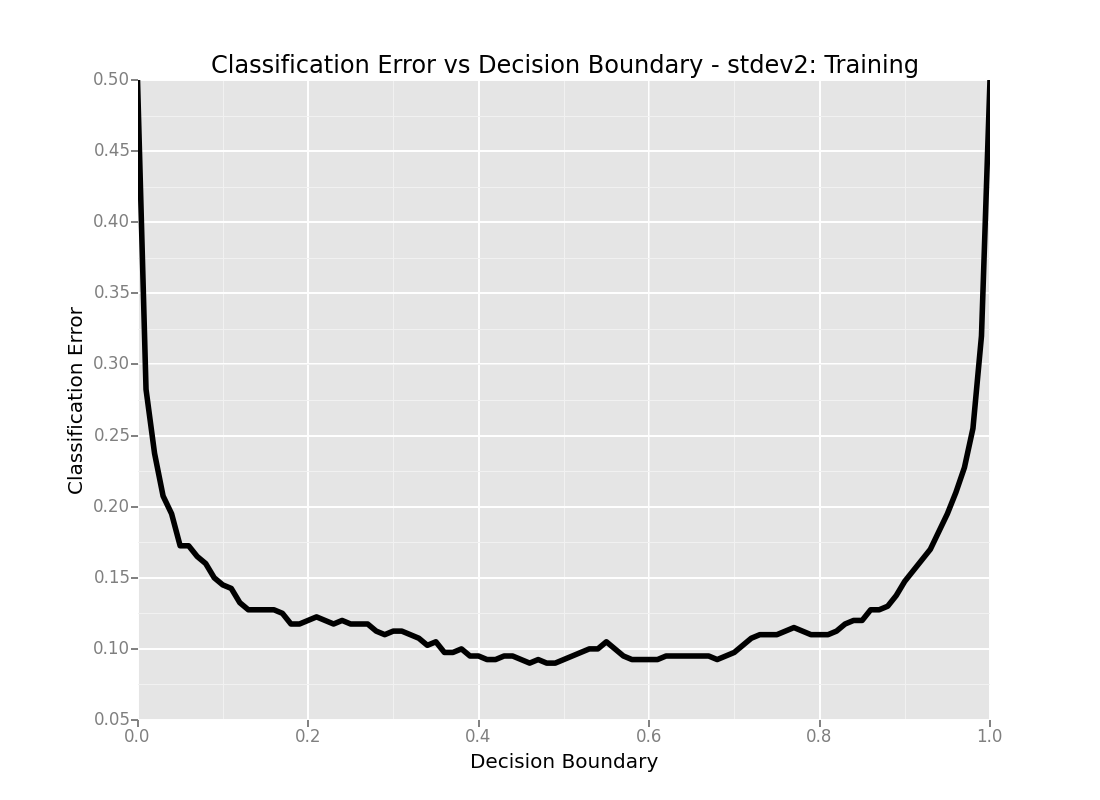
\includegraphics[width=1\linewidth, height=1in]{CEDB_stdev2_train.png}
		\caption*{stdev2 (Training)}
	\end{minipage}
	\begin{minipage}[b]{.24\linewidth}
		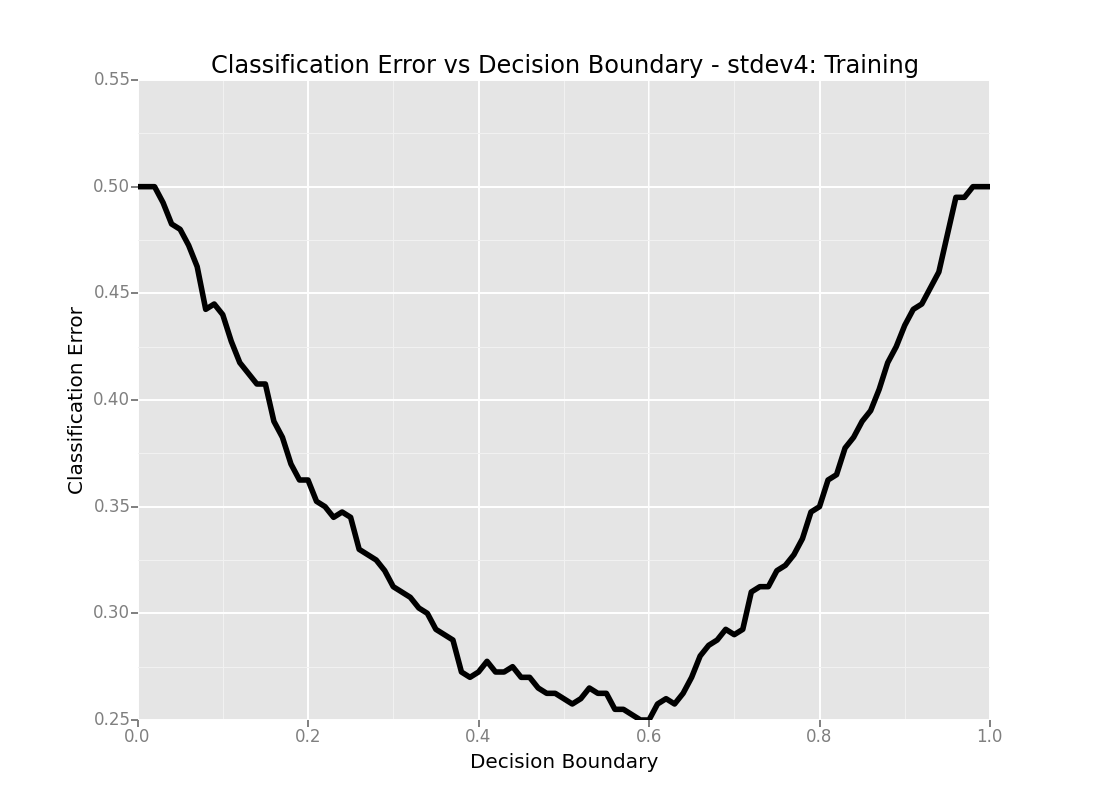
\includegraphics[width=1\linewidth, height=1in]{CEDB_stdev4_train.png}
		\caption*{stdev4 (Training)}
	\end{minipage}
	\begin{minipage}[b]{.24\linewidth}
		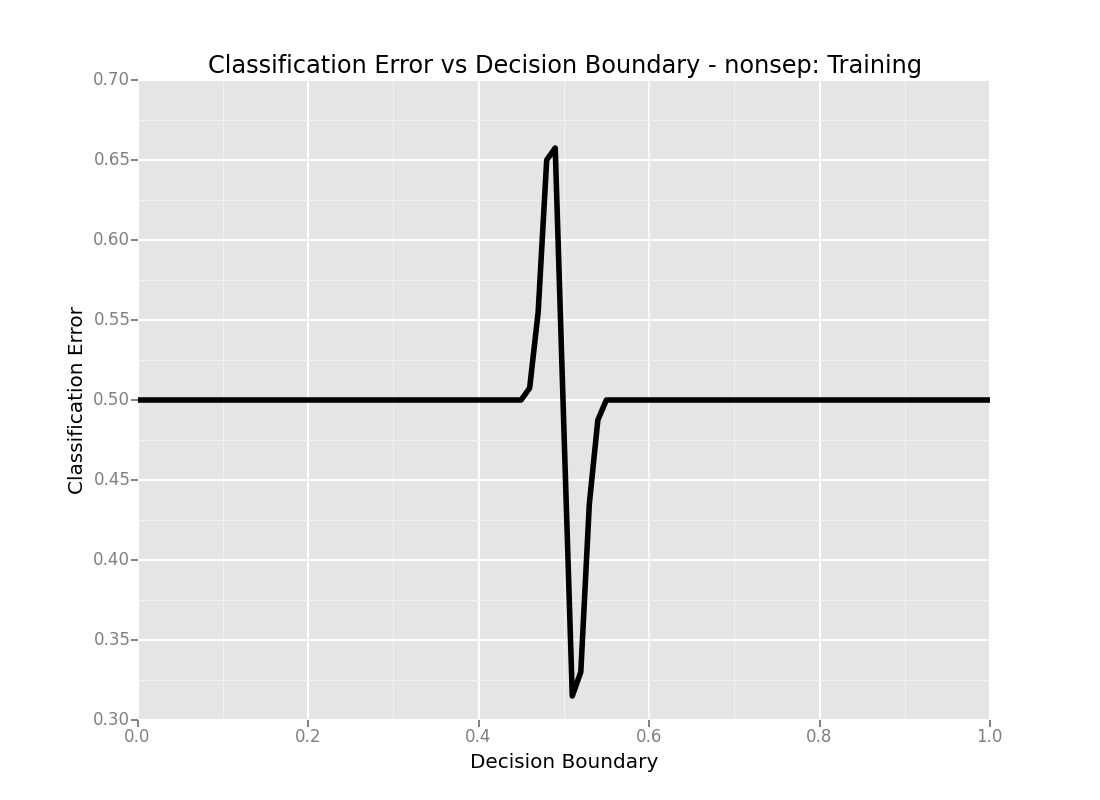
\includegraphics[width=1\linewidth, height=1in]{CEDB_nonsep_train.png}
		\caption*{nonsep (Training)}
	\end{minipage}
		\begin{minipage}[b]{.24\linewidth}
		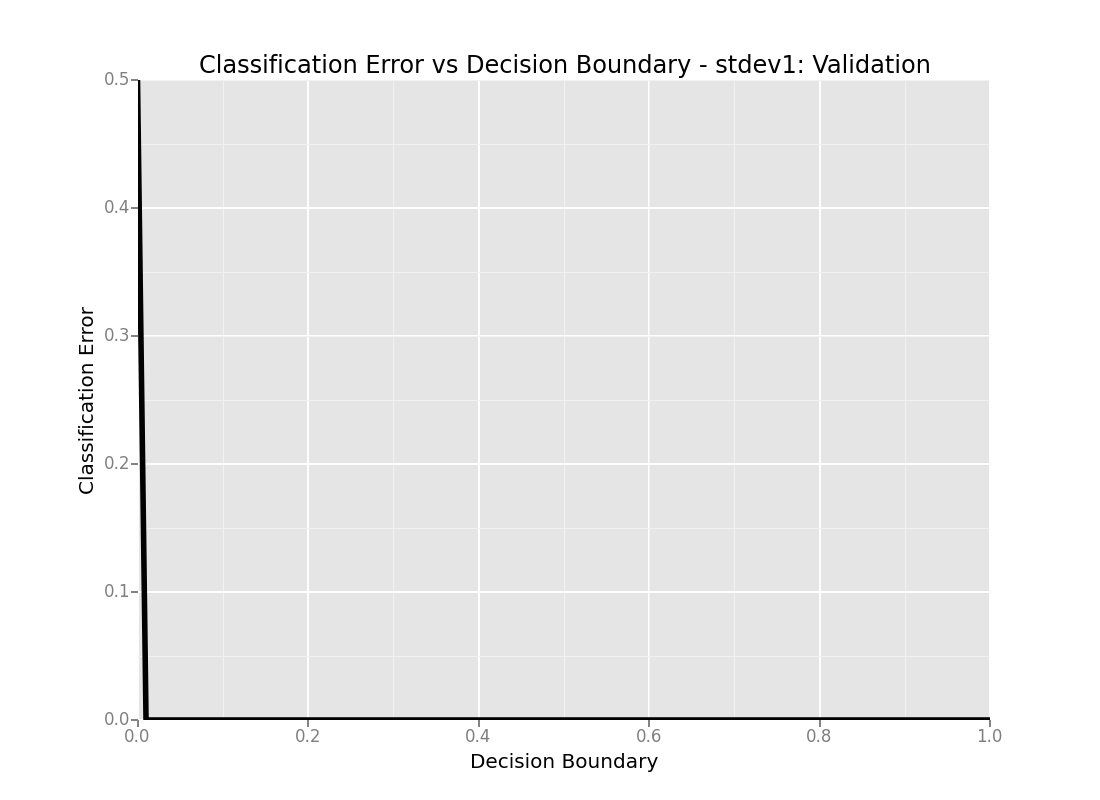
\includegraphics[width=1\linewidth, height=1in]{CEDB_stdev1_validation.png}
		\caption*{stdev1 (Validation)}
	\end{minipage}
	\begin{minipage}[b]{.24\linewidth}
		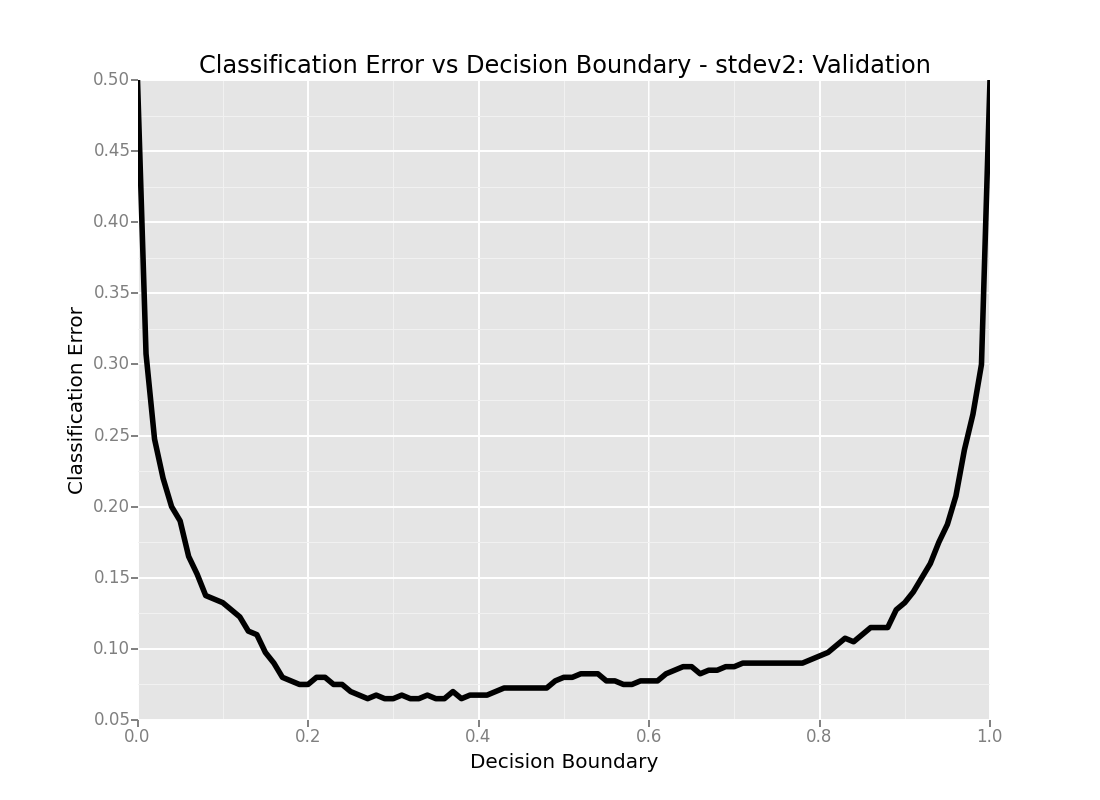
\includegraphics[width=1\linewidth, height=1in]{CEDB_stdev2_validation.png}
		\caption*{stdev2 (Validation)}
	\end{minipage}
	\begin{minipage}[b]{.24\linewidth}
		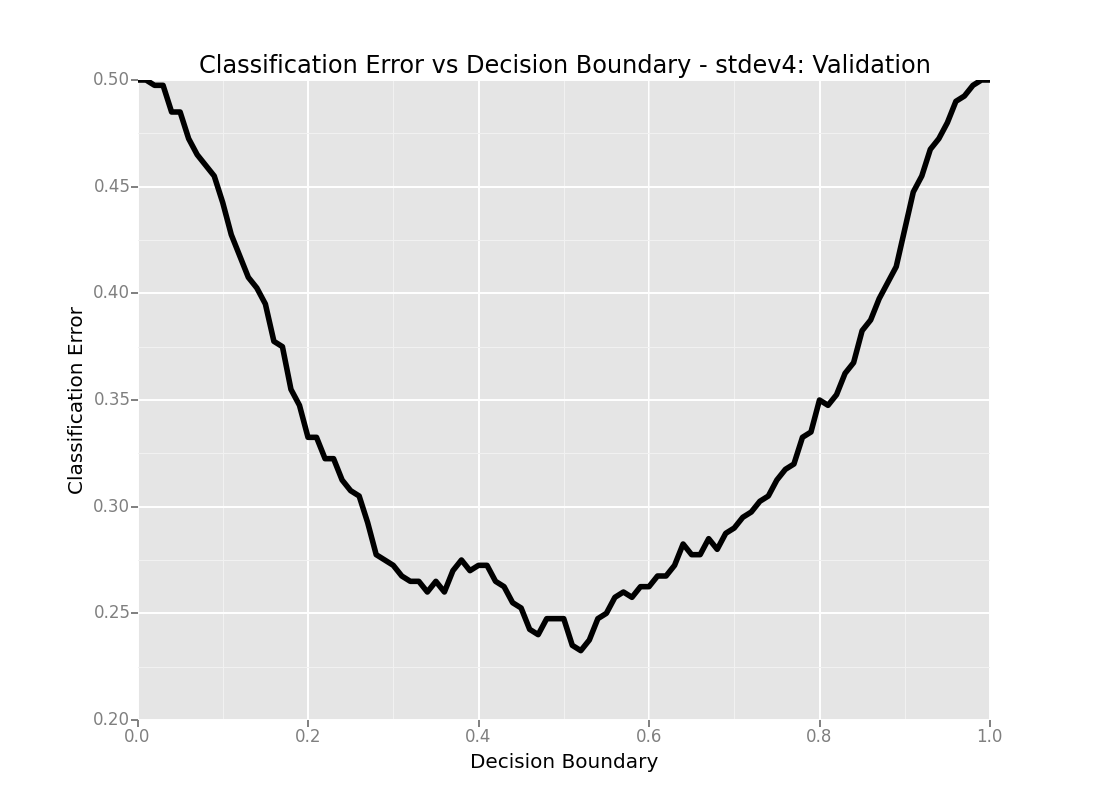
\includegraphics[width=1\linewidth, height=1in]{CEDB_stdev4_validation.png}
		\caption*{stdev4 (Validation)}
	\end{minipage}
	\begin{minipage}[b]{.24\linewidth}
		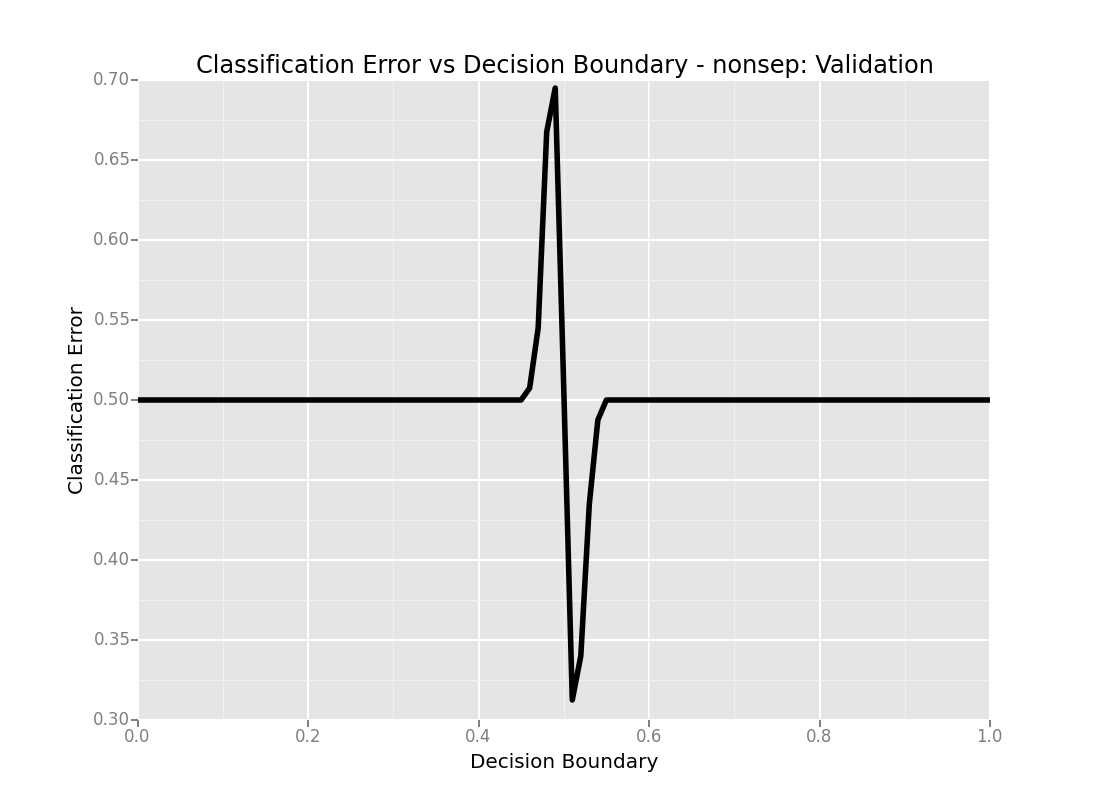
\includegraphics[width=1\linewidth, height=1in]{CEDB_nonsep_validation.png}
		\caption*{nonsep (Validation)}
	\end{minipage}
	\caption{The classification error of Logistic Regression as a function of our choice of a decision boundary for the stdev1, stdev2, stdev4, and nonsep (training and validation) datasets}
\end{figure}

In the linearly separable case (stdev1), we see that just about any value greater than 0 gives us perfect classification, which makes intuitive sense since the optimal weights will try to push everything to either 0 or 1 resulting in the graph we see: the error starts out at .5 and almost immediately drops to 0. However if the data is still generally but not perfectly linearly separable (stdev2 and stdev4), we get what we would expect--classification error starts high and decreases until around decision boundary of 0.5 and then starts to increase again. In the linearly non-seperable case (nonsep), the probabilities are all relatively close to 0.5. Hence we don't see any effect of changing the decision boundary until we get relatively close to 0.5 in this case, we see that we get a spike since we start to misclassify the green points while all the purple points are still incorrectly classified. The spike drops back to 0.5 at around decision boundary of 0.5 and decreases as we start to correctly classify all the purple points. As we continue to increase the decision boundary, we get to the case were we classify everything as purple leading us with a misclassification rate of 0.5. 

We also explore the effect of adding a ridge penalty to logistic regression. We plot the classification error and loss of our regression as a function of the penalty $lambda$:

\begin{figure}[ht]
	\centering
	\begin{minipage}[b]{.24\linewidth}
		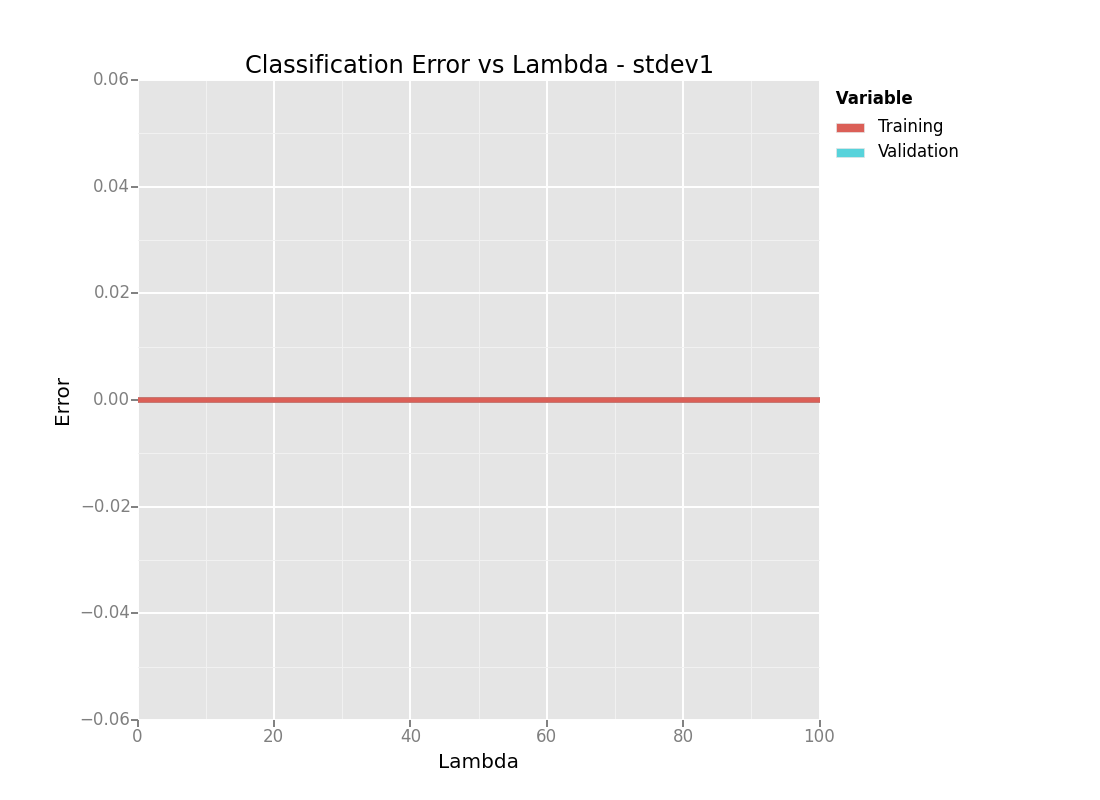
\includegraphics[width=1\linewidth, height=1in]{CErr_lambda_stdev1.png}
		\caption*{Error - stdev1}
	\end{minipage}
	\begin{minipage}[b]{.24\linewidth}
		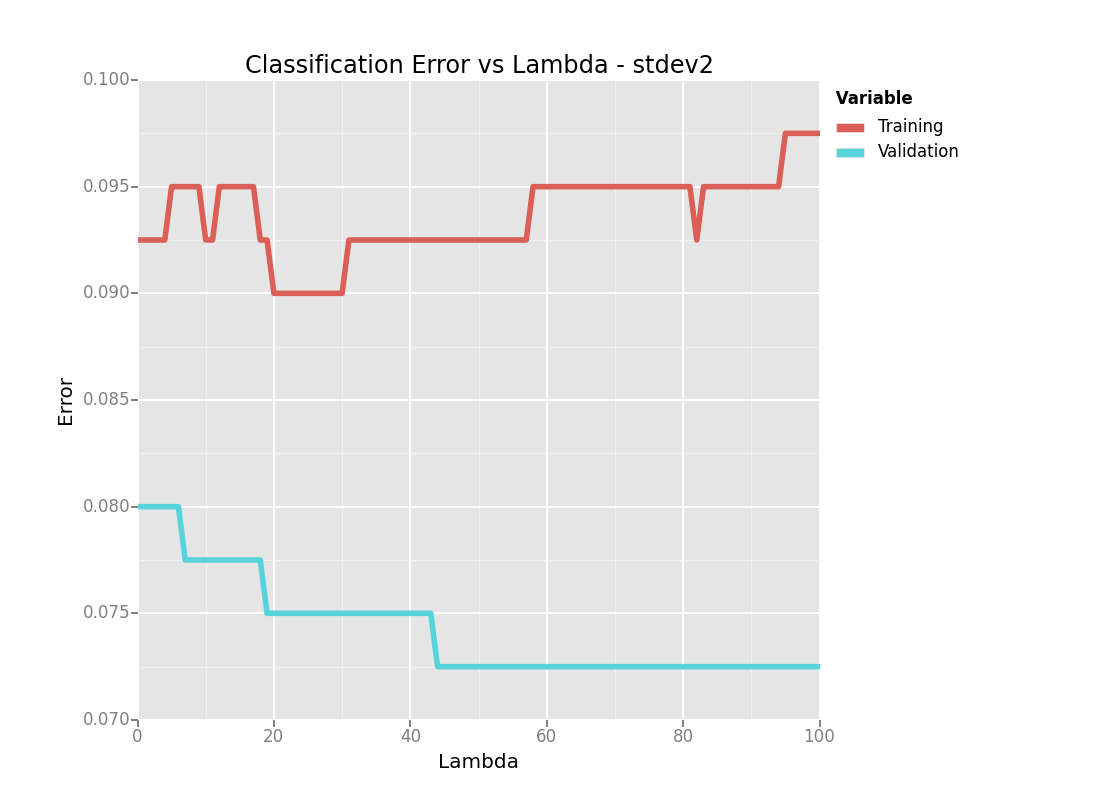
\includegraphics[width=1\linewidth, height=1in]{CErr_lambda_stdev2.png}
		\caption*{Error - stdev2}
	\end{minipage}
	\begin{minipage}[b]{.24\linewidth}
		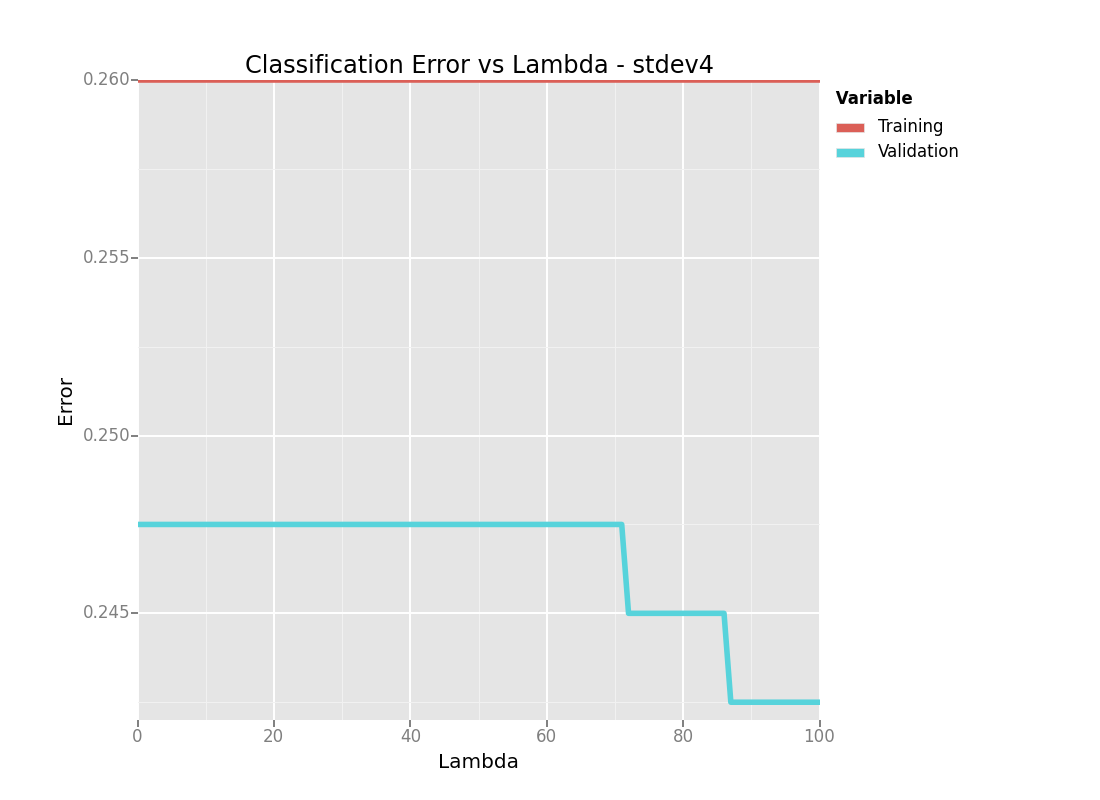
\includegraphics[width=1\linewidth, height=1in]{CErr_lambda_stdev4.png}
		\caption*{Error - stdev4}
	\end{minipage}
	\begin{minipage}[b]{.24\linewidth}
		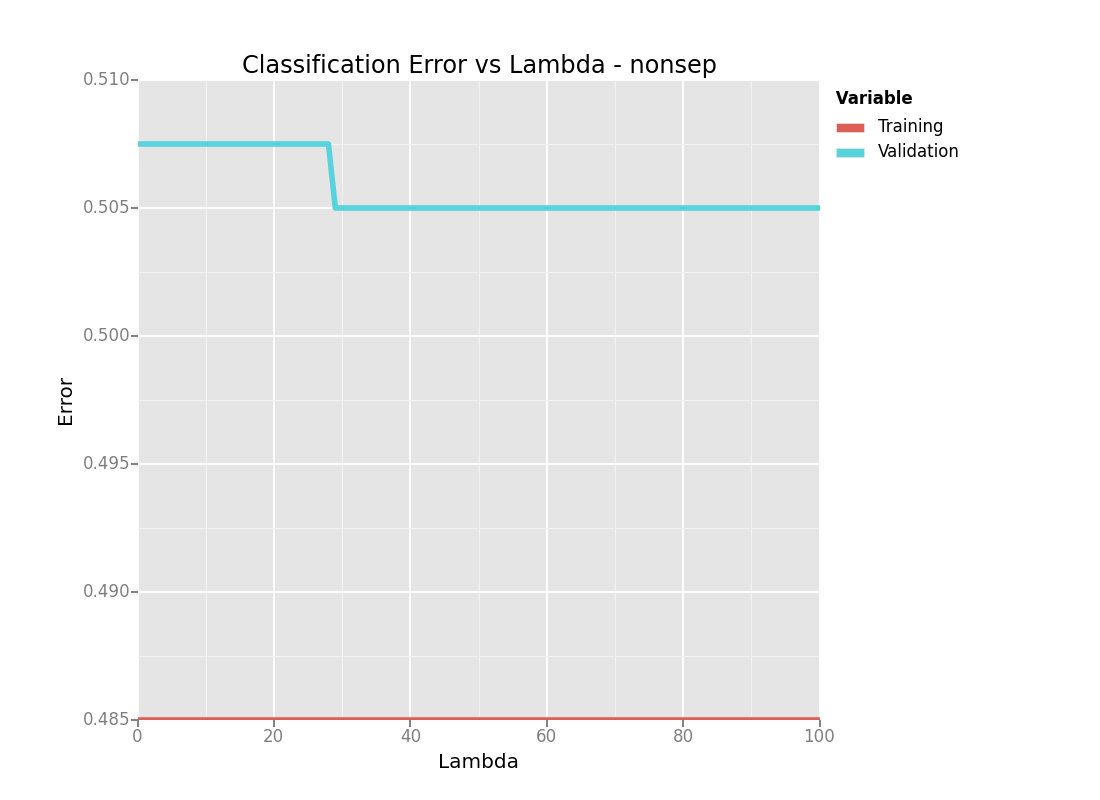
\includegraphics[width=1\linewidth, height=1in]{CErr_lambda_nonsep.png}
		\caption*{Error - nonsep}
	\end{minipage}
		\begin{minipage}[b]{.24\linewidth}
		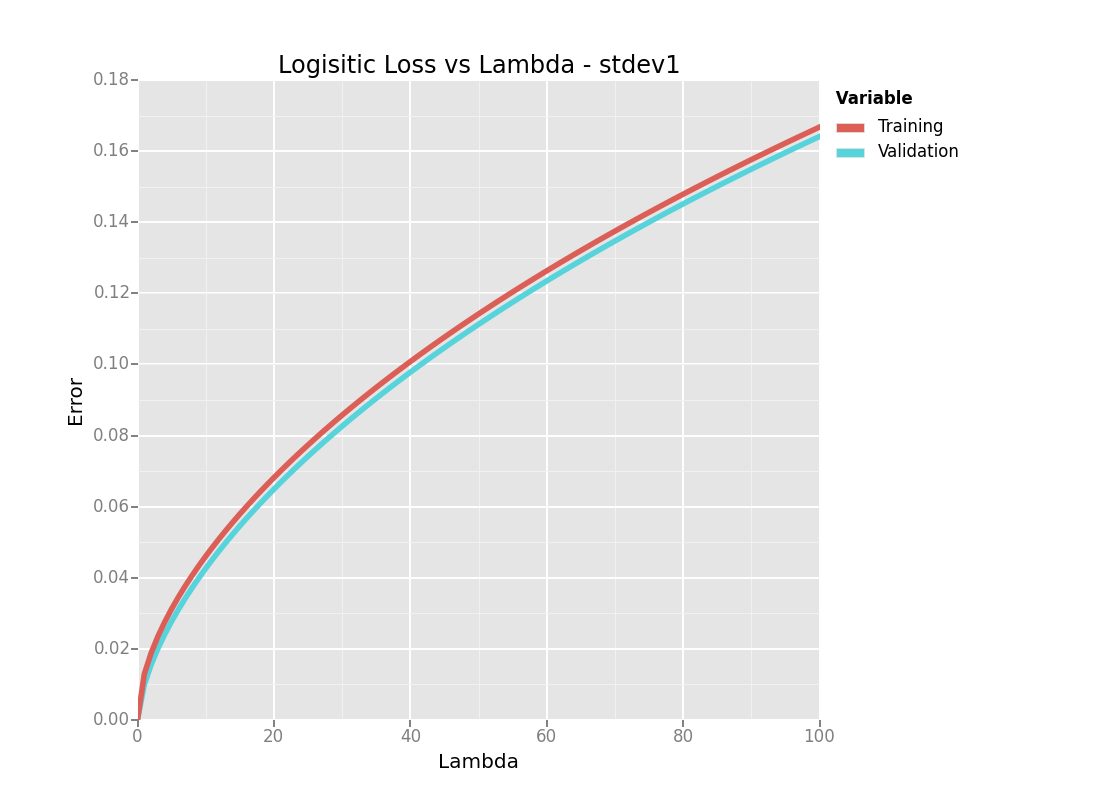
\includegraphics[width=1\linewidth, height=1in]{Loss_lambda_stdev1.png}
		\caption*{Logistic Loss - stdev1}
	\end{minipage}
	\begin{minipage}[b]{.24\linewidth}
		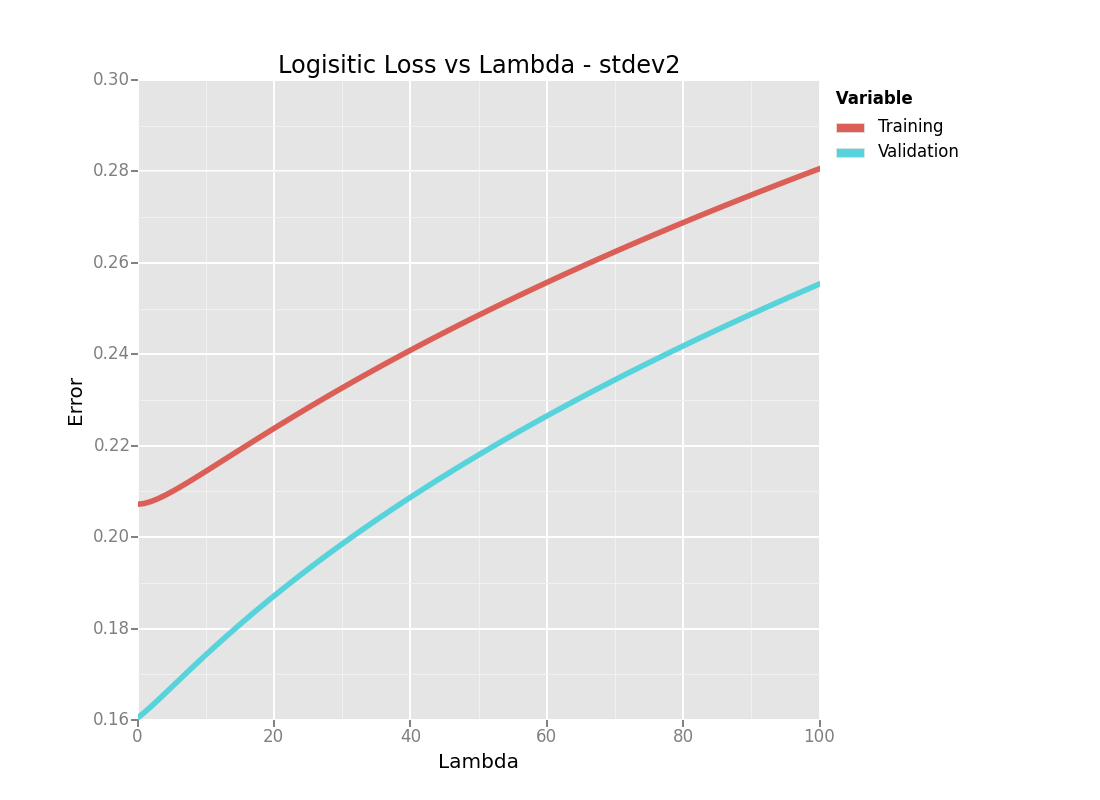
\includegraphics[width=1\linewidth, height=1in]{Loss_lambda_stdev2.png}
		\caption*{Logistic Loss - stdev2}
	\end{minipage}
	\begin{minipage}[b]{.24\linewidth}
		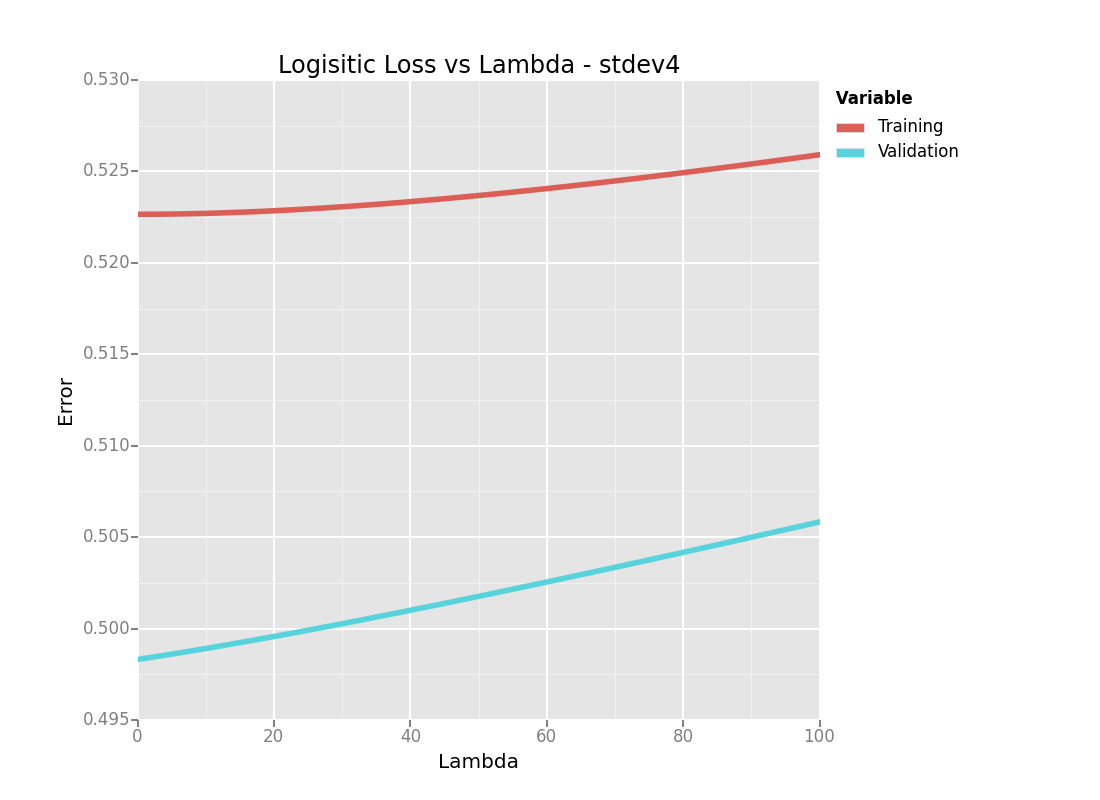
\includegraphics[width=1\linewidth, height=1in]{Loss_lambda_stdev4.png}
		\caption*{Logistic Loss - stdev4}
	\end{minipage}
	\begin{minipage}[b]{.24\linewidth}
		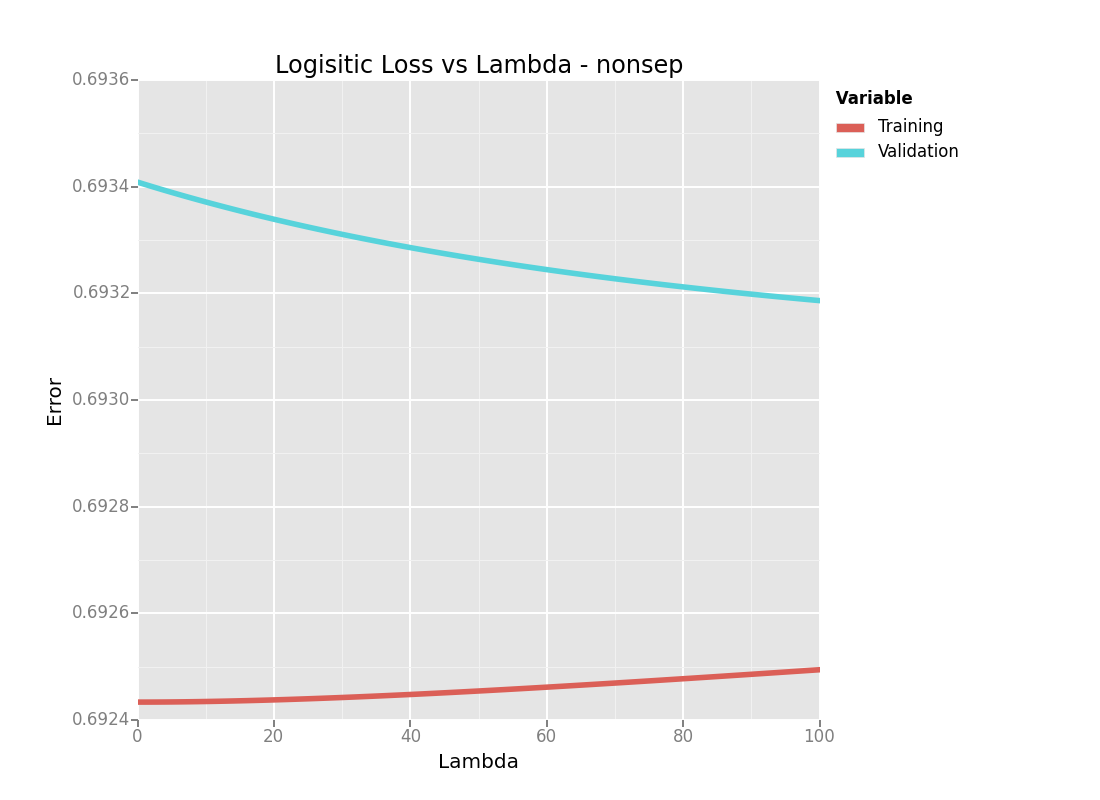
\includegraphics[width=1\linewidth, height=1in]{Loss_lambda_nonsep.png}
		\caption*{Logistic Loss - nonsep}
	\end{minipage}
	\caption{Classification Error (for a decision boundary of 0.5) and Loss of Logistic Regression as a function of the L2 penalty $\lambda$}
\end{figure}

We see that generally speaking, the classification error on the validation set decreases (except in the linearly separable case, where it stays at 0) as we increase our ridge penalty which is something we might expect if we think there's possible overfitting. We also see that generally speaking, loss monotonically increases with lambda, something we should expect since the ridge penalty is pushing the weights toward 0 causing logistic regression to output probabilities closer to 0.5.

\subsubsection*{Support Vector Machines}

Let's now compare the performance of SVM to that of logistic regression for classification problems. To illustrate the objective and constraints of the support vector machine, we have included below the explicit objective we would optimize over, as well as the constraints, for the dual form of a linear SVM with slack variables. The equations below correspond to the 2D problem where we have positive examples (1, 2), (2, 2) and negative examples (0, 0), (-2, 3).

\[
\min_{\alpha_1, \alpha_2, \alpha_3, \alpha_4}
\frac{1}{2}
\begin{bmatrix}
    \alpha_1 & \alpha_2 & \alpha_3 & \alpha_4 \\
\end{bmatrix}
\begin{bmatrix}
    5       & 6 & 0 & -4 \\
    6       & 8 & 0 & -2 \\
    0       & 0 & 0 & 0 \\
    -4       & -2 & 0 & 13 \\
\end{bmatrix}
\begin{bmatrix}
    \alpha_1 \\
    \alpha_2 \\
    \alpha_3 \\
    \alpha_4 \\
\end{bmatrix} 
+
\begin{bmatrix}
    -1       & -1 & -1 & -1 \\
\end{bmatrix}
\begin{bmatrix}
    \alpha_1 \\
    \alpha_2 \\
    \alpha_3 \\
    \alpha_4 \\
\end{bmatrix} 
\]

\begin{center}
s.t.
\end{center}

\[
\begin{bmatrix}
    -1 & 0 & 0 & 0 \\
    0 & -1 & 0 & 0 \\
    0 & 0 & -1 & 0 \\
    0 & 0 & 0 & -1 \\
    1 & 0 & 0 &0 \\
    0 & 1 & 0 & 0 \\
    0 & 0 & 1 & 0 \\
    0 & 0 & 0 & 1 \\
\end{bmatrix}
\begin{bmatrix}
    \alpha_1 \\
    \alpha_2 \\
    \alpha_3 \\
    \alpha_4 \\
\end{bmatrix} 
\leq
\begin{bmatrix}
0 \\
0 \\ 
0 \\ 
0 \\ 
C \\
C \\ 
C \\ 
C \\
\end{bmatrix},
\]

\[
\begin{bmatrix}
    1 & 1 & -1 & -1 \\
\end{bmatrix}
\begin{bmatrix}
    \alpha_1 \\
    \alpha_2 \\
    \alpha_3 \\
    \alpha_4 \\
\end{bmatrix} 
= 0
\]

\begin{table}
\captionof{table}{Performance of Linear SVM on provided data sets}
\begin{tabular}{llllll}
\toprule
{} & dataset & classification error rate (training set) & classification error rate (validation set) \\
\midrule
  & data\_stdev1 & 0.00\% & 0.00\% \\
  & data\_stdev2 & 9.50\% & 7.50\% \\
  & data\_stdev4 & 26.00\% & 23.50\% \\
  & data\_nonsep & 49.50\% & 51.25\% \\
\bottomrule
\end{tabular}
\end{table}

\begin{figure}[ht]
	\centering
	\begin{minipage}[b]{.24\linewidth}
		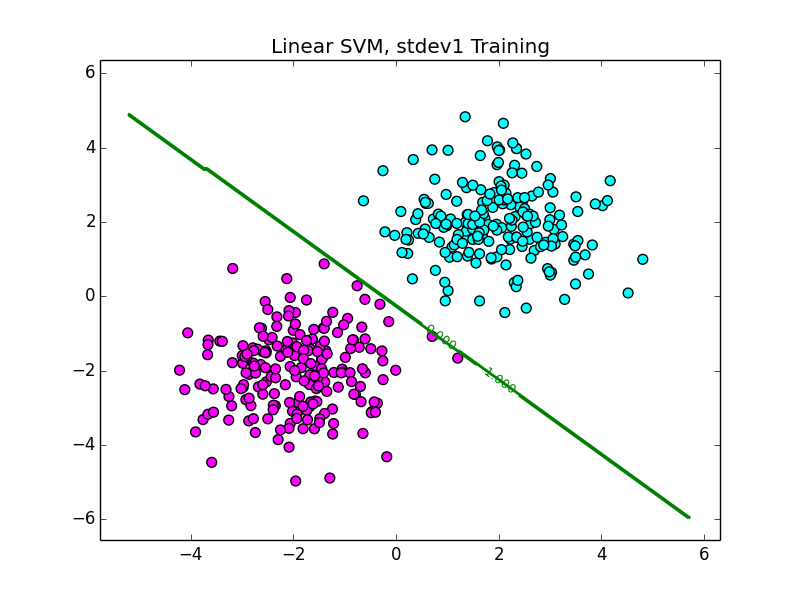
\includegraphics[width=1\linewidth, height=1in]{linear_svm_stdev1_train.png}
		\caption*{stdev1 (Training)}
	\end{minipage}
	\begin{minipage}[b]{.24\linewidth}
		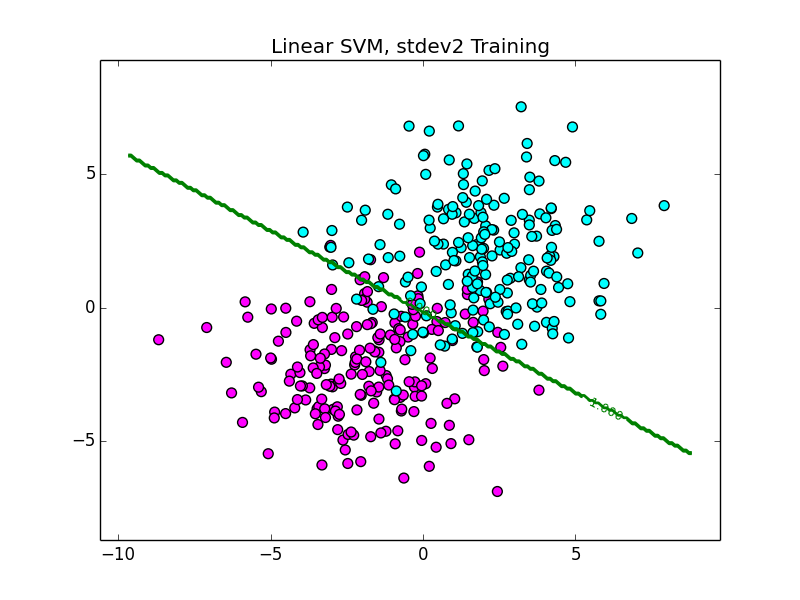
\includegraphics[width=1\linewidth, height=1in]{linear_svm_stdev2_train.png}
		\caption*{stdev2 (Training)}
	\end{minipage}
	\begin{minipage}[b]{.24\linewidth}
		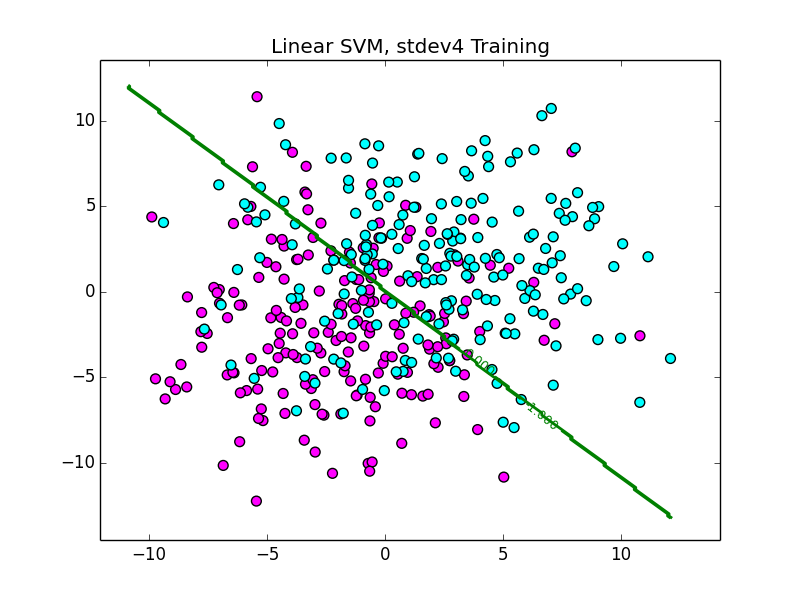
\includegraphics[width=1\linewidth, height=1in]{linear_svm_stdev4_train.png}
		\caption*{stdev4 (Training)}
	\end{minipage}
	\begin{minipage}[b]{.24\linewidth}
		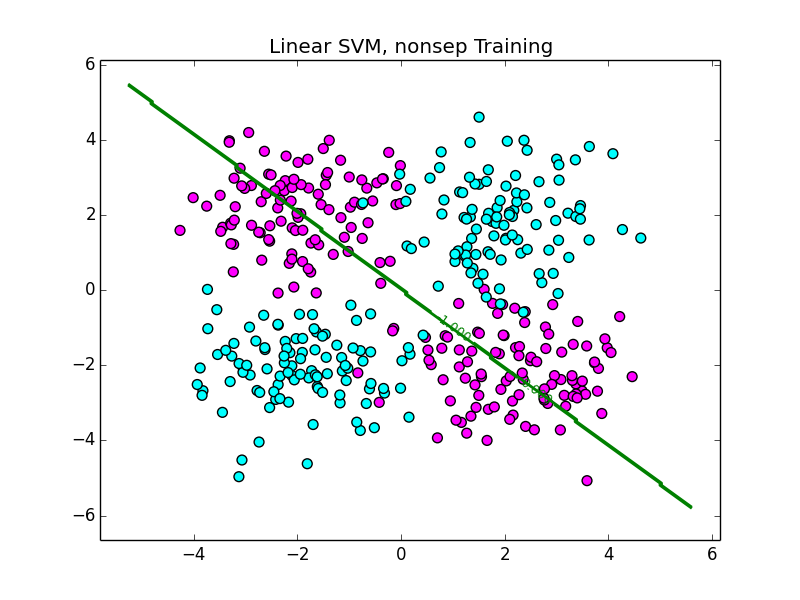
\includegraphics[width=1\linewidth, height=1in]{linear_svm_nonsep_train.png}
		\caption*{nonsep (Training)}
	\end{minipage}
		\begin{minipage}[b]{.24\linewidth}
		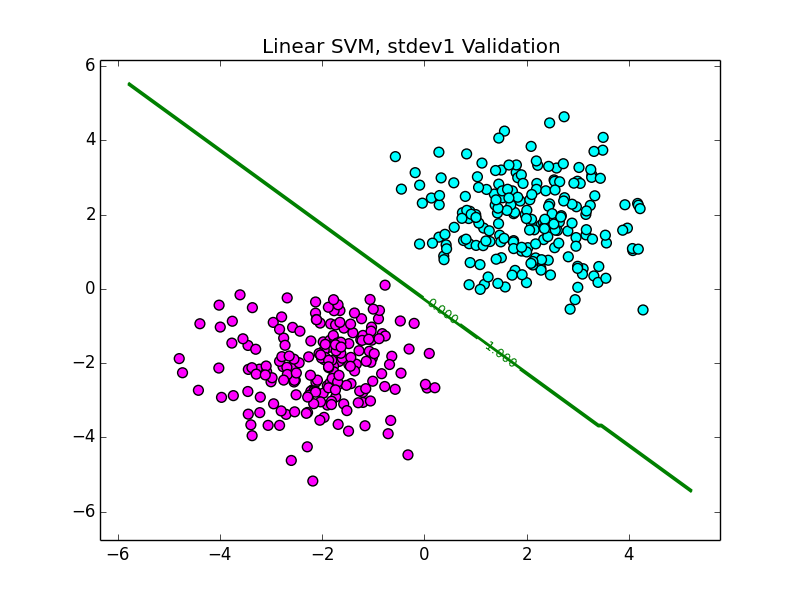
\includegraphics[width=1\linewidth, height=1in]{linear_svm_stdev1_validation.png}
		\caption*{stdev1 (Validation)}
	\end{minipage}
	\begin{minipage}[b]{.24\linewidth}
		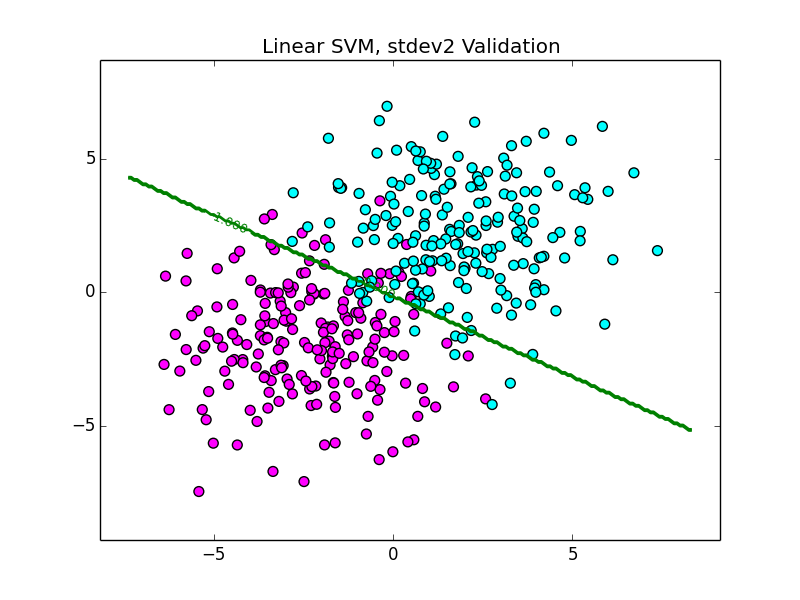
\includegraphics[width=1\linewidth, height=1in]{linear_svm_stdev2_validation.png}
		\caption*{stdev2 (Validation)}
	\end{minipage}
	\begin{minipage}[b]{.24\linewidth}
		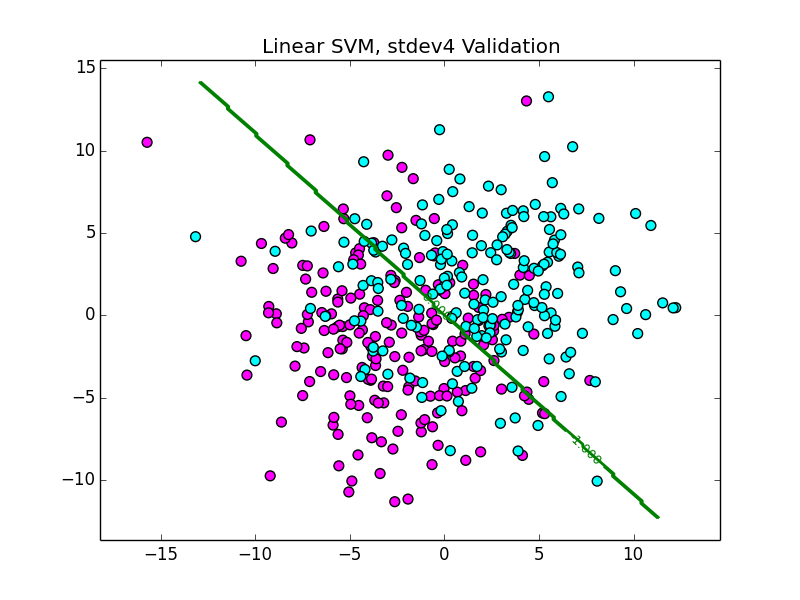
\includegraphics[width=1\linewidth, height=1in]{linear_svm_stdev4_validation.png}
		\caption*{stdev4 (Validation)}
	\end{minipage}
	\begin{minipage}[b]{.24\linewidth}
		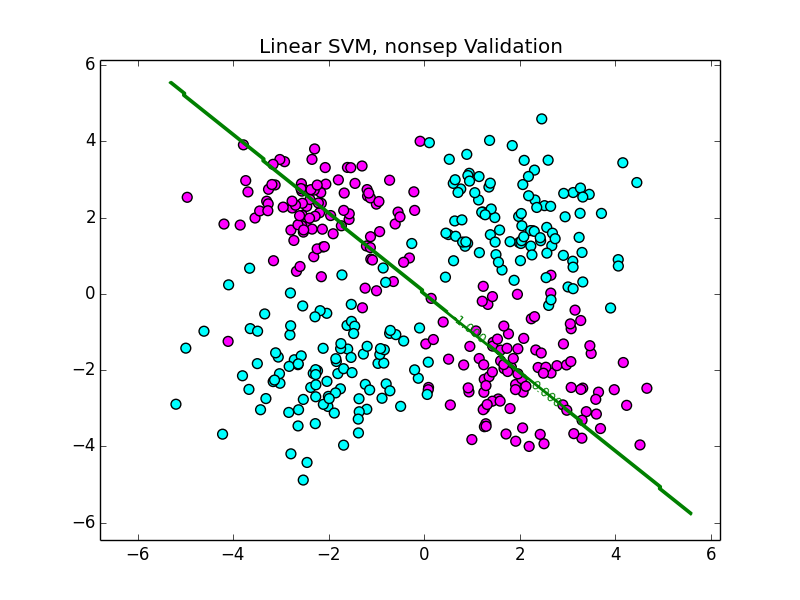
\includegraphics[width=1\linewidth, height=1in]{linear_svm_nonsep_validation.png}
		\caption*{nonsep (Validation)}
	\end{minipage}
	\caption{The decision boundaries generated by SVM plotted against the stdev1, stdev2, stdev4, and nonsep (training and validation) datasets}
\end{figure}

\subsubsection*{Titanic Data}
We're interesting in now testing the performance of our classifiers on a real dataset. In this case, we are using the Titanic dataset where we're doing the rather macabre task of trying to predict passenger survival given his or her features. So this problem we first scale all the features so they lie between $[0,1]$. WE accomplish by taking each observation and transforming it via:
\begin{equation*}
	x_{i,j}^* = \frac{x_{i,j}-\min(x_j)}{\max(x_j) - \min(x_j)}
\end{equation*}
We scale our data in such a way so our logistic regression behaves nicely. Otherwise, we encounter precision loss errors that end up significantly impacting our predictive accuracy. 

Using this transformed data, we train a logistic regression, a linear SVM, a polynomial SVM ($K(x,z) = (1+x\cdot z)^3$), and a gaussian SVM. For each classifier, we perform a grid search to choose the optimal hyperparameters that minimize the classification error of the validation set. We find that for:
\begin{itemize}
	\item Logistic Regression, $\lambda = 0.38$
	\item Linear SVM, $C = 0.07$
	\item Polynomial SVM, $C=0.03$
	\item Gaussian SVM, $\sigma = 1$ and $C=0.04$
\end{itemize} 

With these settings we obtain the following results:
\begin{table}[ht]
\centering
\captionof{table}{Titanic Data Classification Performance}
\begin{tabular}{lrrrr}
\toprule
{} & Logit & L-SVM & P-SVM & G-SVM \\
\midrule
Penalty & $\lambda = 0.38$ & $C = 0.07$ & $C = 0.03$ & $C = 0.04$\\
\midrule
Training Error    &  0.165 &  0.225 & 0.140 &  0.195 \\
Validation Error  &  0.208 &  0.208 & 0.222 &  0.210 \\
Test Error        &  0.249 &  0.233 & 0.265 &  0.243 \\
Geometric Margin  & {}     &  0.0055& 0.0112& 0.0063 \\
\bottomrule
\end{tabular}	
\end{table}

\begin{table}[ht]
\centering
\captionof{table}{Optimal Weight Table}
\begin{tabular}{lrrrr}
\toprule
{} & Logit & L-SVM & P-SVM & G-SVM \\
\midrule
Penalty & $\lambda = 0.38$ & $C = 0.07$ & $C = 0.03$ & $C = 0.04$\\
\midrule
$w_1$  &  0.603693 &  0.031302 & -0.012892 &  0.120059 \\
$w_2$  &  0.455286 &  0.033952 & -0.010501 &  0.255103 \\
$w_3$  & -1.058978 & -0.065245 &  0.023511 & -0.375139 \\
$w_4$  &  2.475588 &  1.901134 &  0.101932 &  1.440000 \\
$w_5$  & -0.914359 & -0.078502 & -0.009049 & -0.068269 \\
$w_6$  & -0.251056 & -0.011503 &  0.000163 & -0.036648 \\
$w_7$  &  0.538155 &  0.131051 &  0.010683 &  0.104903 \\
$w_8$  &  0.330644 &  0.057787 & -0.001549 &  0.117515 \\
$w_9$  & -0.233114 & -0.038255 & -0.009864 & -0.159978 \\
$w_{10}$ &  0.291611 &  0.029324 &  0.024844 &  0.240000 \\
$w_{11}$ & -0.058496 &  0.008941 & -0.014863 & -0.080000 \\
\bottomrule
\end{tabular}	
\end{table}

\end{document}